\begin{center}
\LARGE Appendices
\end{center}
\appendix

\paragraph{Outline}

This paper gathers all the supplementary material and goes as follows: \Cref{sec:proofs} details all the proofs of the main results. \Cref{sec:risk-sensitive-supp} and \Cref{sec:bftq-full} recall respectively the scalable \BFTQ algorithm and the risk-sensitive exploration procedure. \Cref{sec:lagragian} describes a naive alternative to \BFTQ based on Lagrangian Relaxation. The \Cref{sec:exp-supp} assembles all the assets for visualising and reproducing the experiments, including visualisations of policy executions, algorithms and environment parameters, and instructions for executing the attached source code. Finally we fill the Machine Learning Reproducibility Checklist and we justify each statement in \Cref{sec:ml-checklist}.





\section{Proofs of Main Results}
\label{sec:proofs}
\subsection{\Cref{prop:bellman-expectation}}

\begin{proof}
This proof is the same as that in classical multi-objective MDPs.

\begin{align*}
    V^\pi(\os) &\eqdef \expectedvalue\left[ G^\pi \condbar \ov{s_0} = \os\right] \\
    &=\sum_{\oa\in\ocA} \probability{\oa_0 = \oa \condbar\ov{s_0} = \os} \expectedvalue\left[ G^\pi \condbar \ov{s_0} = \os, \oa_0 = \oa\right]\\
    &= \sum_{\oa\in\ocA} \pi(\oa | \os) Q^\pi(\os,\oa)
\end{align*}
\begin{align*}
    Q^\pi(\os, \oa) &\eqdef \expectedvalue\left[\sum_{t=0}^\infty \gamma^t R(\os_t, \oa_t)\condbar \ov{s_0} = \os, \ov{a_0} = \oa\right] \\
    &= R(\os, \oa) + \sum_{\os'\in\ocS}\probability{\os_1 = \os' \condbar\ov{s_0} = \os, \ov{a_0} = \oa}\cdot \expectedvalue\left[\sum_{t=1}^\infty \gamma^t R(\os_t, \oa_t)\condbar \ov{s_1} = \os'\right] \\
    &= R(\os, \oa) + \gamma\sum_{\os'\in\ocS}\ov{P}\left(\os' \condbar\os, \oa\right) \expectedvalue\left[\sum_{t=0}^\infty \gamma^t R(\os_t, \oa_t) \condbar \ov{s_0} = \os'\right] \\
    &=  R(\os, \oa) + \gamma\sum_{\os'\in\ocS}\ov{P}\left(\os' \condbar\os, \oa\right) V^\pi(\os')
\end{align*}

\textbf{Contraction of $\cT^\pi$:}
Let $\pi\in\Pi, Q_1, Q_2\in(\Real^2)^{\ocS\ocA}$.
\begin{align*}
    \forall \os\in\ocS, \oa\in\ocA,\quad \left|\cT^\pi Q_1(\os,\oa) - \cT^\pi Q_2(\os,\oa)\right| &= \left|\gamma\expectedvalueover{\substack{\os'\sim\ov{P}(\os'|\os,\oa) \\ \oa'\sim\pi(\oa'|\os')}} Q_1(\os',\oa') - Q_2(\os',\oa')\right|\\
    &\leq \gamma\left\|Q_1-Q_2\right\|_\infty
\end{align*}
Hence, $\left\|\cT^\pi Q_1  - \cT^\pi Q_2 \right\|_\infty \leq \gamma\left\|Q_1-Q_2\right\|_\infty$

According to the Banach fixed point theorem, $\cT^\pi$ admits a unique fixed point.
It can be easily verified that $Q^\pi$ is indeed this fixed point by combining the two Bellman Expectation equations \eqref{eq:bellman_expectation}.

\end{proof}

\subsection{\Cref{thm:bellman-optimality}}

\begin{proof}
Let $\os, \oa \in \ocA\times\ocS$. For this proof, we consider  potentially non-stationary policies $\pi=(\rho, \pi')$, with $\rho\in\cM(\ocA)$, $\pi'\in\cM(\ocA)^\Natural$. The results will apply to the particular case of stationary optimal policies, when they exist.

\begin{align}
    Q_r^*(\os, \oa) &=  \max_{\rho, \pi'} Q_r^{\rho, \pi'}(\os', \oa') \label{eq:pthm_def}\\
    &= \max_{\rho, \pi'} R_r(\os, \oa) + \gamma \sum_{\os'\in\cS} P(\os' | \os, \oa) V_r^{\rho, \pi'}(\os') \label{eq:pthm_exp}\\
    &= R_r(\os, \oa) + \gamma \sum_{\os'\in\cS}  P(\os' | \os, \oa) \max_{\rho, \pi'} \sum_{\oa'\in\ocA} \rho(\oa' | \os')Q_r^{\pi'}(\os', \oa') \label{eq:pthm_marg}\\
    &= R_r(\os, \oa) + \gamma \sum_{\os'\in\cS}  P(\os' | \os, \oa) \max_\rho\sum_{\oa'\in\ocA}\rho(\oa' | \os')\max_{\pi'\in\Pi_a(\os')}Q_r^{\pi'}(\os', \oa') \label{eq:pthm_max}\\
    &= R_r(\os, \oa) + \gamma \sum_{\os'\in\cS}  P(\os' | \os, \oa) \max_\rho\expectedvalueover{\oa'\sim\rho}Q_r^*(\os', \oa') \label{eq:pthm_marg_def2}
\end{align}
where $\pi = (\rho, \pi')\in\Pi_a(\os)$ and $\pi'\in\Pi_a(\os')$.

This follows from:
\begin{enumerate}
\item[\eqref{eq:pthm_def}.] Definition of $Q^*$. 
\item[\eqref{eq:pthm_exp}.] Bellman Expectation expansion from \Cref{prop:bellman-expectation}.
\item[\eqref{eq:pthm_marg}.] Marginalisation on $\oa'$.
\item[\eqref{eq:pthm_max}.] \begin{itemize}
    \item Trivially $\max_{\pi'\in\Pi_a(\os')} \sum_{\oa'\in\cA} \cdot \leq \sum_{\oa'\in\cA} \max_{ \pi'\in\Pi_a(\os)} \cdot$
    \item Let $\ov{\pi}\in\argmax_{\pi'\in\Pi_a(\os')} Q_r^{\pi'}(\os', \oa')$, then:
    \begin{align*}
        \sum_{\oa'\in\ov{A}}\rho(\oa'|\os')\max_{\pi'\in\Pi_a(\os')}Q_r^{\pi'}(\os', \oa') &= \sum_{\oa'\in\ov{A}}\rho(\oa'|\os')Q_r^{\ov{\pi}}(\os', \oa') \\
        &\leq  \max_{\pi'\in\Pi_a(\os')} \sum_{\oa'\in\ov{A}}\rho(\oa'|\os')Q_r^{\pi'}(\os', \oa')
    \end{align*}
\end{itemize}
\item[\eqref{eq:pthm_marg_def2}.] Definition of $Q^*$.
\end{enumerate}

Moreover, the condition $\pi=(\rho, \pi')\in\Pi_a(\os)$ gives
\begin{equation*}
   \expectedvalueover{\oa'\sim\rho} Q_c^{*}(\os, \oa) = \expectedvalueover{\oa'\sim\rho} Q_c^{\pi'}(\os, \oa) = V_c^{\pi}(\os) \leq \beta
\end{equation*}

Consequently, $\pi_\text{greedy}(\cdot; Q^*)$ belongs to the $\argmax$ of \eqref{eq:pthm_marg_def2}, and in particular:
\begin{equation*}
     Q_r^*(\os, \oa) = r(\os, \oa) + \gamma \sum_{\os'\in\cS}  P(\os' | \os, \oa) \expectedvalueover{\oa'\sim\pi_\text{greedy}(\os', Q^*)} Q_r^*(\os', \oa')
\end{equation*}

The same reasoning can be made for $Q_c^*$ by replacing $\max$ operators by $\min$, and $\Pi_a$ by $\Pi_r$.
\end{proof}


\subsection{\Cref{prop:greedy_optimal}}
\begin{proof}
Notice from the definitions of $\cT$ and $\cT^\pi$ in \eqref{eq:bellman-optimality} and \eqref{eq:bellman_expectation_operator} that $\cT$ and $\cT^{\pi_\text{greedy}(\cdot;Q^*)}$ coincide on $Q^*$. Moreover, since $Q^* = \cT Q^*$ by \Cref{thm:bellman-optimality}, we have: $    \cT^{\pi_\text{greedy}(\cdot;Q^*)} Q^* = \cT Q^* = Q^*
$.
Hence, $Q^*$ is a fixed point of $\cT^{\pi_\text{greedy}(\cdot;Q^*)}$, and by \Cref{prop:bellman-expectation} it must be equal to $Q^{\pi_\text{greedy}(\cdot;Q^*)}$

To show the same result for $V^*$, notice that 
\begin{equation*}
    V^{\pi_\text{greedy}(Q^*)}(\os) = \expectedvalueover{\oa\sim\pi_\text{greedy}(Q^*)}Q^{\pi_\text{greedy}(Q^*)}(\os,\oa) = \expectedvalueover{\oa\sim\pi_\text{greedy}(Q^*)}Q^*(\os,\oa)
\end{equation*}
By applying the definitions of $Q^*$ and $\pi_\text{greedy}$, we recover the definition of $V^*$.
\end{proof}

\subsection{\Cref{thm:contraction}}
\label{sec:proof_contraction}
\begin{proof}
In the trivial case $|\cA| = 1$, there exits only one policy $\pi$ and $\cT = \cT^\pi$, which is a contraction by \Cref{prop:bellman-expectation}.

In the general case $|\cA| \geq 2$, we can build the following counter-example:

Let $(\cS, \cA, P, R_r, R_c)$ be a BMDP.
For any $0 < \epsilon < 1$, we define $Q_\epsilon^1$ and $Q_\epsilon^2$ as:

\begin{align*}
      Q_\epsilon^1(\os,\oa) =
      \begin{cases}
    (0, 1), & \text{if } a = a_0 \\
    (\frac{1}{\epsilon}, 1+\epsilon), & \text{if } a \neq a_0
  \end{cases}\\
  Q_\epsilon^2(\os,\oa) =
      \begin{cases}
    (1, 0), & \text{if } a = a_0 \\
    (1+\frac{1}{\epsilon}, \epsilon), & \text{if } a \neq a_0
  \end{cases}
\end{align*}
Then, $\|Q_1-Q_2\|_\infty = 1$.
 $Q_\epsilon^1$ and $Q_\epsilon^2$ are represented in \Cref{fig:concavity_example}.

\begin{figure}[tp]
    \centering
    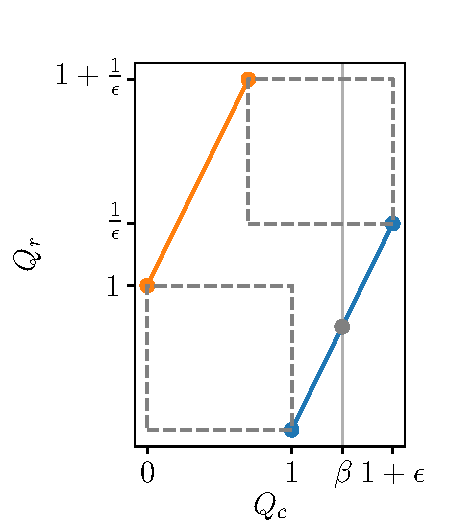
\includegraphics[width=0.5\textwidth]{source/img/concavity_example.pdf}
    \caption{Representation of $Q_\epsilon^1$ (blue) and $Q_\epsilon^2$ (yellow)}
    \label{fig:concavity_example}
\end{figure}

But for $\oa=(a,\beta_a)$ with $\beta_a = 1+\epsilon/2$, we have:
\begin{align*}
    \|\cT Q_\epsilon^1(\os, \oa) - \cT Q_\epsilon^2(\os, \oa)\|_\infty &= \gamma\left\|\expectedvalueover{\os'\sim\ov{P}(\os'|\os,\oa)} \expectedvalueover{\oa'\sim\pi_\text{greedy}(Q^1_\epsilon)}Q^1_\epsilon(\os',\oa') - \expectedvalueover{\oa'\sim\pi_\text{greedy}(Q^2_\epsilon)}Q^2_\epsilon(\os',\oa')\right\|_\infty \\
    &= \gamma\left\|\expectedvalueover{\os'\sim\ov{P}(\os'|\os,\oa)}(\frac{1}{2\epsilon}, 1+\frac{\epsilon}{2}) - (1+\frac{1}{\epsilon},\epsilon )\right\|_\infty \\
    &= \gamma(1+\frac{1}{2\epsilon})
\end{align*}
Hence, $\|\cT Q_\epsilon^1 - \cT Q_\epsilon^2\|_\infty \geq \gamma(1+\frac{1}{2\epsilon})$

As a conclusion, there does not exist $L>0$ such that:
$$\forall Q_1,Q_2\in(\Real^2)^{\ocS\ocA}, \|\cT Q^1 - \cT Q^2\|_\infty \leq L \|Q^1 - Q^2\|_\infty$$
In other words, $\cT$ is not a contraction for $\|\cdot\|_\infty$.
\end{proof}

\subsection{\Cref{rmk:contractivity-smooth}}
\label{proof:contraction-with-smooth}
\begin{proof}
We now study the contractivity of $\cT$ when restricted to the functions of $\cL_\gamma$ defined as follows:
\begin{equation}
    \cL_\gamma = \left\{\begin{array}{cc}
         Q\in(\Real^2)^{\ocS\ocA}\text{ s.t. }\exists L<\frac{1}{\gamma}-1: \forall \os\in\ocS,\oa_1,\oa_2\in\ocA,   \\
         |Q_r(\os,\oa_1) - Q_r(\os,\oa_2)| \leq L|Q_c(\os,\oa_1) - Q_c(\os,\oa_2)|
    \end{array}\right\}
\end{equation}
That is, for all state $\os$, the set $Q(\os, \ocA)$ plot in the $(Q_c,Q_r)$ plane must be the \emph{graph} of a $L$-Lipschitz function, with $L<1/\gamma-1$.

We impose such structure for the following reason: the counter-example presented above prevented contraction because it was a pathological case in which the slope of $Q$ can be arbitrary large. As a consequence, when solving $Q_r^*$ such that $Q_c^*=\beta$, a vertical slice of a $\|\cdot\|_\infty$ ball around $Q_1$ (which must contain $Q_2$) can be arbitrary large as well.

This sketch of proof makes use of insights detailed in the proof of \Cref{prop:bftq_pi_hull}, which we recommend the reader to consult first.

We denote $\cB(Q,R)$ the ball of centre $Q$ and radius $R$ for the $\|\cdot\|_\infty$-norm:
\begin{equation*}
    \cB(Q,R) = \{Q'\in(R^2)^{\ocS\ocA}: \|Q-Q'\|_\infty \leq R\}
\end{equation*}

We give the three main steps required to show that $\cT$ restricted to $\cL_\gamma$ is a contraction. Given $Q^1, Q^2\in\cL_\gamma$, show that:
\begin{enumerate}
    \item $Q^2\in\cB(Q^1,R)\implies\cF^2\in\cB(\cF^1, R), \forall\os\in\ocS$, where $\cF$ is the top frontier of the convex hull of undominated points, as defined in \Cref{sec:proof_pi_hull}.
    \item $Q\in\cL_\gamma \implies \cF$ is the graph of a $L$-Lipschitz function, $\forall\os\in\ocS$.
    \item taking the slice $Q_c=\beta$ of a ball $\cB(\cF,R)$ with $\cF$ $L$-Lipschitz results in an interval on $Q_r$ of range at most $(L+1)R$
\end{enumerate}

These three steps will allow us to control $Q_r^{2*} - Q_r^{1*}$ as a function of $R = \|Q^2-Q^1\|_\infty$.

\textbf{Step 1:} we want to show that if $Q^1$ and $Q^2$ are close, then $\cF^1$ are $\cF^2$ are close as well in the following sense:
\begin{align}
    \cF^2\in\cB(\cF^1, R) &\iff d(\cF^1, \cF^2) \leq R \iff \max_{q^2\in\cF^2}\min_{q^1\in\cF^1}\|q^2-q^1\|_\infty \leq R
    \label{eq:ball-set}
\end{align}
Assume $Q^2\in\cB(Q^1,R)$.
We start by showing this result for $\cC^2(Q^{1-})$ and $\cC^2(Q^{2-})$ as defined in \Cref{sec:proof_pi_hull}:

Let $\os\in\ocS$ and $q^2\in\cC^2(Q^{2-})$, $\exists\lambda\in[0,1], \oa_1,\oa_2\in\ocA: q^2 = (1-\lambda)Q^2(\os,\oa_1) + \lambda Q^2(\os,\oa_2)$. Define $q^1 = (1-\lambda)Q^1(\os,\oa_1) + \lambda Q^1(\os,\oa_2)$. Then 
\begin{align*}
    \|q^2-q^1\|_\infty &= \|(1-\lambda)(Q^2(\os,\oa_1) - Q^1(\os,\oa_1)) + \lambda (Q^2(\os,\oa_2) - Q^1(\os,\oa_2))\|_\infty\\
    &\leq  (1-\lambda)\|Q^2(\os,\oa_1) - Q^1(\os,\oa_1)\|_\infty + \lambda \|Q^2(\os,\oa_2) - Q^1(\os,\oa_2)\|_\infty\\
    &\leq (1-\lambda)R+\lambda R = R
\end{align*}

It remains to show that when taking the top frontiers of the convex sets $\cC^2(Q^{1-})$ and $\cC^2(Q^{2-})$, they remain at a distance of at most $R$.

This is illustrated in \Cref{fig:contraction_lips_hull}: given a function $Q^1$, we show the locus $\cB(Q_1,R)$ of $Q^2$. We then draw $\cF^1$ the top frontier of the convex hull of $Q^1$ and alongside the locus of all possible $\cF^2$, which belong to a ball $\cB(\cF^1, R)$. 

\begin{figure}[ht]
    \centering
    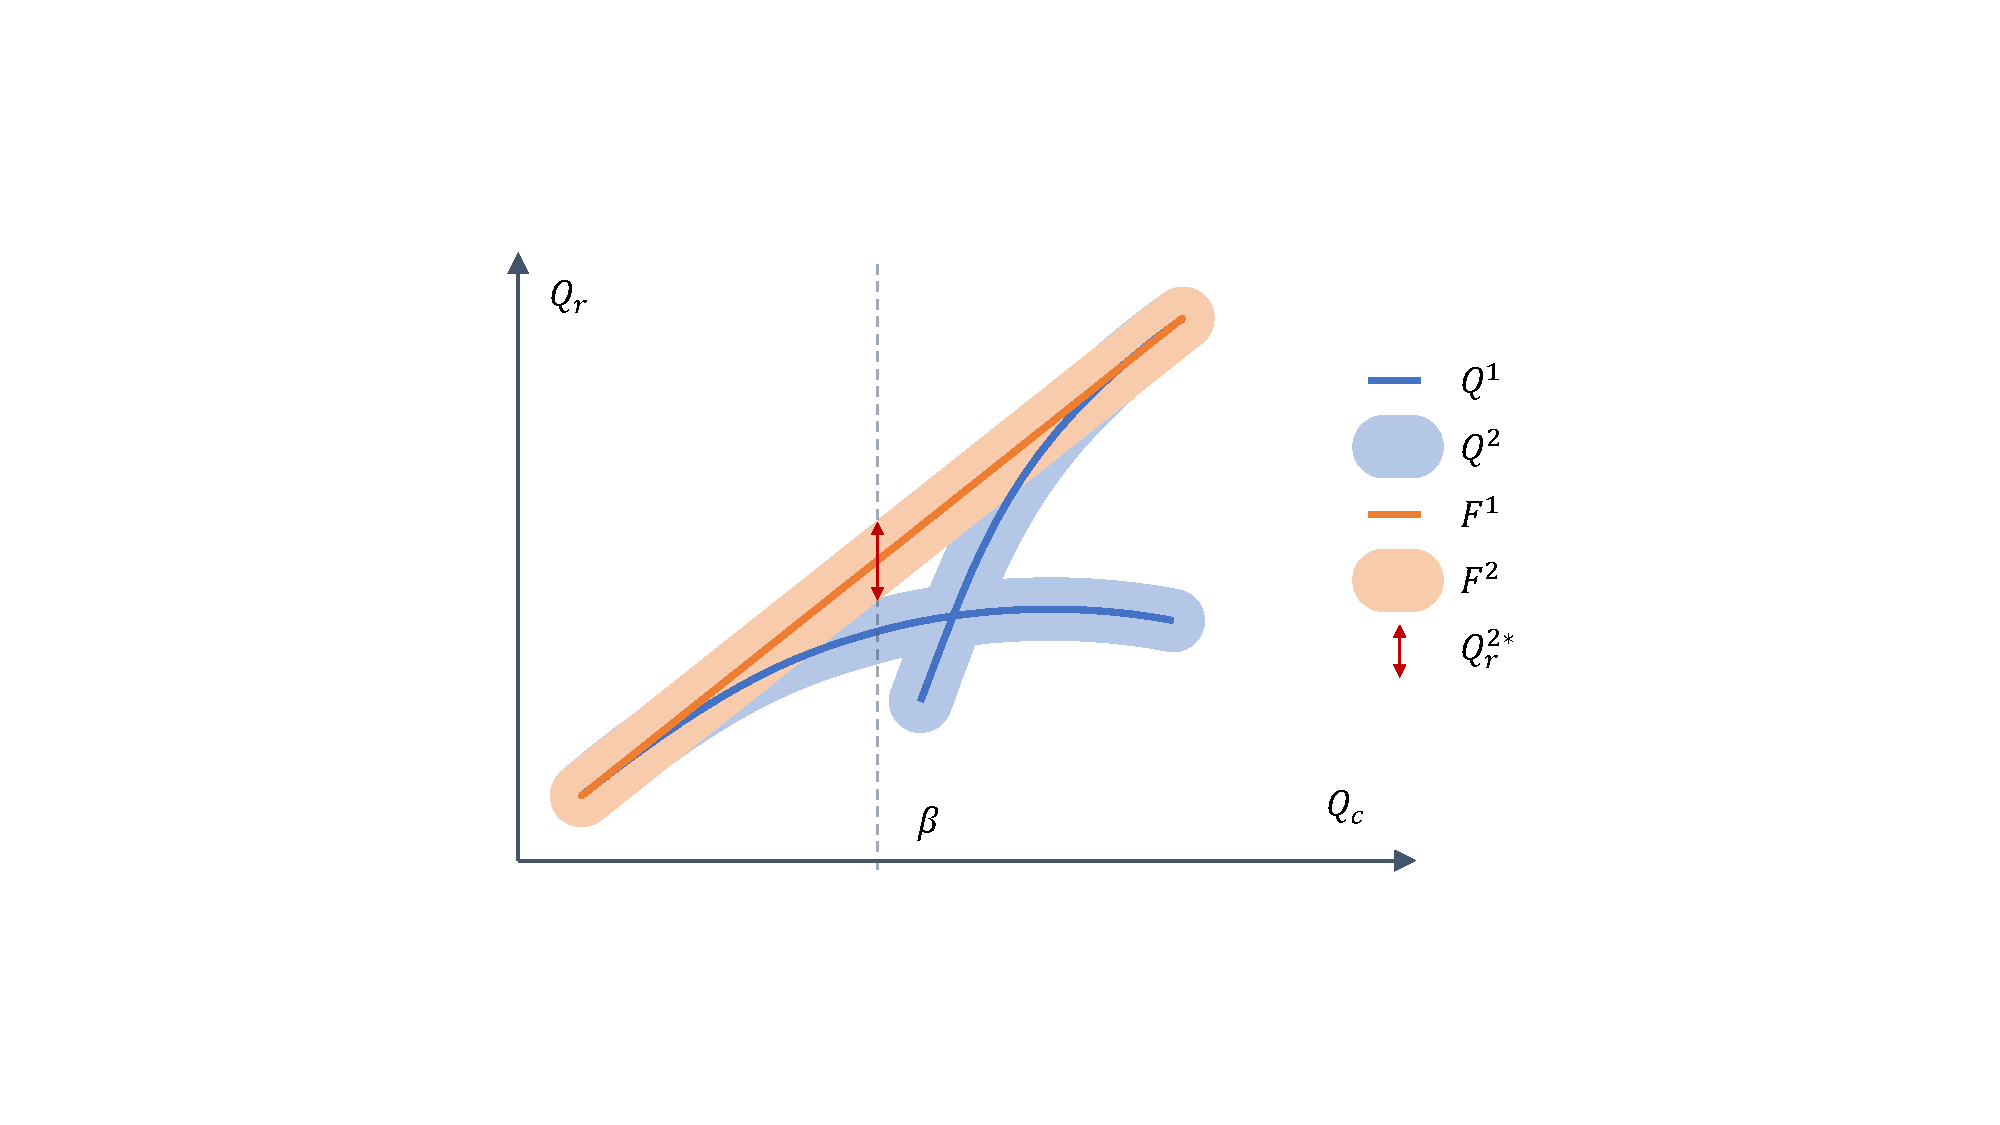
\includegraphics[trim=7cm 4cm 7cm 4cm, clip, width=0.7\textwidth]{source/img/contraction_lipschitz.pdf}
    \caption{We represent the range of possible solutions $Q_r^{2,*}$ for any $Q^2\in\cB(Q^1)$, given $Q_1\in\cL_\lambda$}
    \label{fig:contraction_lips_hull}
\end{figure}

\textbf{Step 2:} We want to show that if $Q\in\cL_\gamma$, $\cF$ is the graph of an $L$-Lipschitz function:
\begin{equation}
\label{eq:L-lip-set}
    \forall q^1,q^2\in\cF, |q_r^2-q_r^1| \leq |q_c^2-q_c^1|
\end{equation}

Let $Q\in\cL_\gamma$ and $\os\in\ocS$, $\cF$ the corresponding top frontier of convex hull.
For all $q^1,q^2\in\cF, \exists \lambda,\mu\in[0,1], q^{11},q^{12},q^{21},q^{22}\in Q(\os,\ocA)$ such that $q^1 = (1-\lambda)q^{11} + \lambda q^{12}$ and $q^2 = (1-\mu)q^{21} + \mu q^{22}$.
Without loss of generality, we can assume $q_c^{11}\leq q_c^{12}$ and $q_c^{21}\leq q_c^{22}$. We also consider the worst case in terms of maximum $q_r$ deviation: $q_c^{12} \leq q_c^{21}$.
Then the maximum increment $q_r^2-q_r^{1}$ is:
\begin{align*}
    \|q^2_r-q^{1}_r\| &\leq \|q^{12}_r-q^{1}_r\| + \|q^{21}_r-q^{12}_r\| + \|q^{2}_r-q^{21}_r\| \\
    &= (1-\lambda)\|q^{12}_r-q^{11}_r\| + \|q^{21}_r-q^{12}_r\| + \mu\|q^{22}_r-q^{21}_r\| \\ 
    &\leq (1-\lambda)L\|q^{12}_c-q^{11}_c\| + L\|q^{21}_c-q^{12}_c\| + \mu L\|q^{22}_c-q^{21}_c\| \\
    &= L\|q^{12}_c-q^{1}_c\| + L\|q^{21}_c-q^{12}_c\| + L\|q^{2}_c-q^{21}_c\|\\
    &= L\|q^{2}_c-q^{1}_c\|
\end{align*}

This can also be seen in \Cref{fig:contraction_lips_hull}: the maximum slope of the $\cF^1$ is lower than the maximum slope between two points of $Q^1$.

\textbf{Step 3:} Let $\cF_1$ be a L-Lipschitz set as defined in \eqref{eq:L-lip-set}, and consider a ball $\cB(\cF_1,R)$ around it as defined in \eqref{eq:ball-set}.

We want to bound the optimal reward value $Q_r^{2*}$ under constraint $Q_c^{2*} = \beta$ (regular case in \Cref{sec:proof_pi_hull} where the constraint is saturated), for any $\cF^2\in\cB(\cF_1,R)$. This quantity is represented as a red double-ended arrow in \Cref{fig:contraction_lips_hull}.

Because we are only interested in what happens locally at $Q_c=\beta$, we can zoom in on \Cref{fig:contraction_lips_hull} and only consider a thin $\epsilon$-section around $\beta$. In the limit $\epsilon\rightarrow 0$, this section becomes the tangent to $\cF^1$ at $Q_c^1=\beta$. It is represented in \Cref{fig:contraction_lips_hull_slope}, from which we derive a geometrical proof:
\begin{figure}[ht]
    \centering
    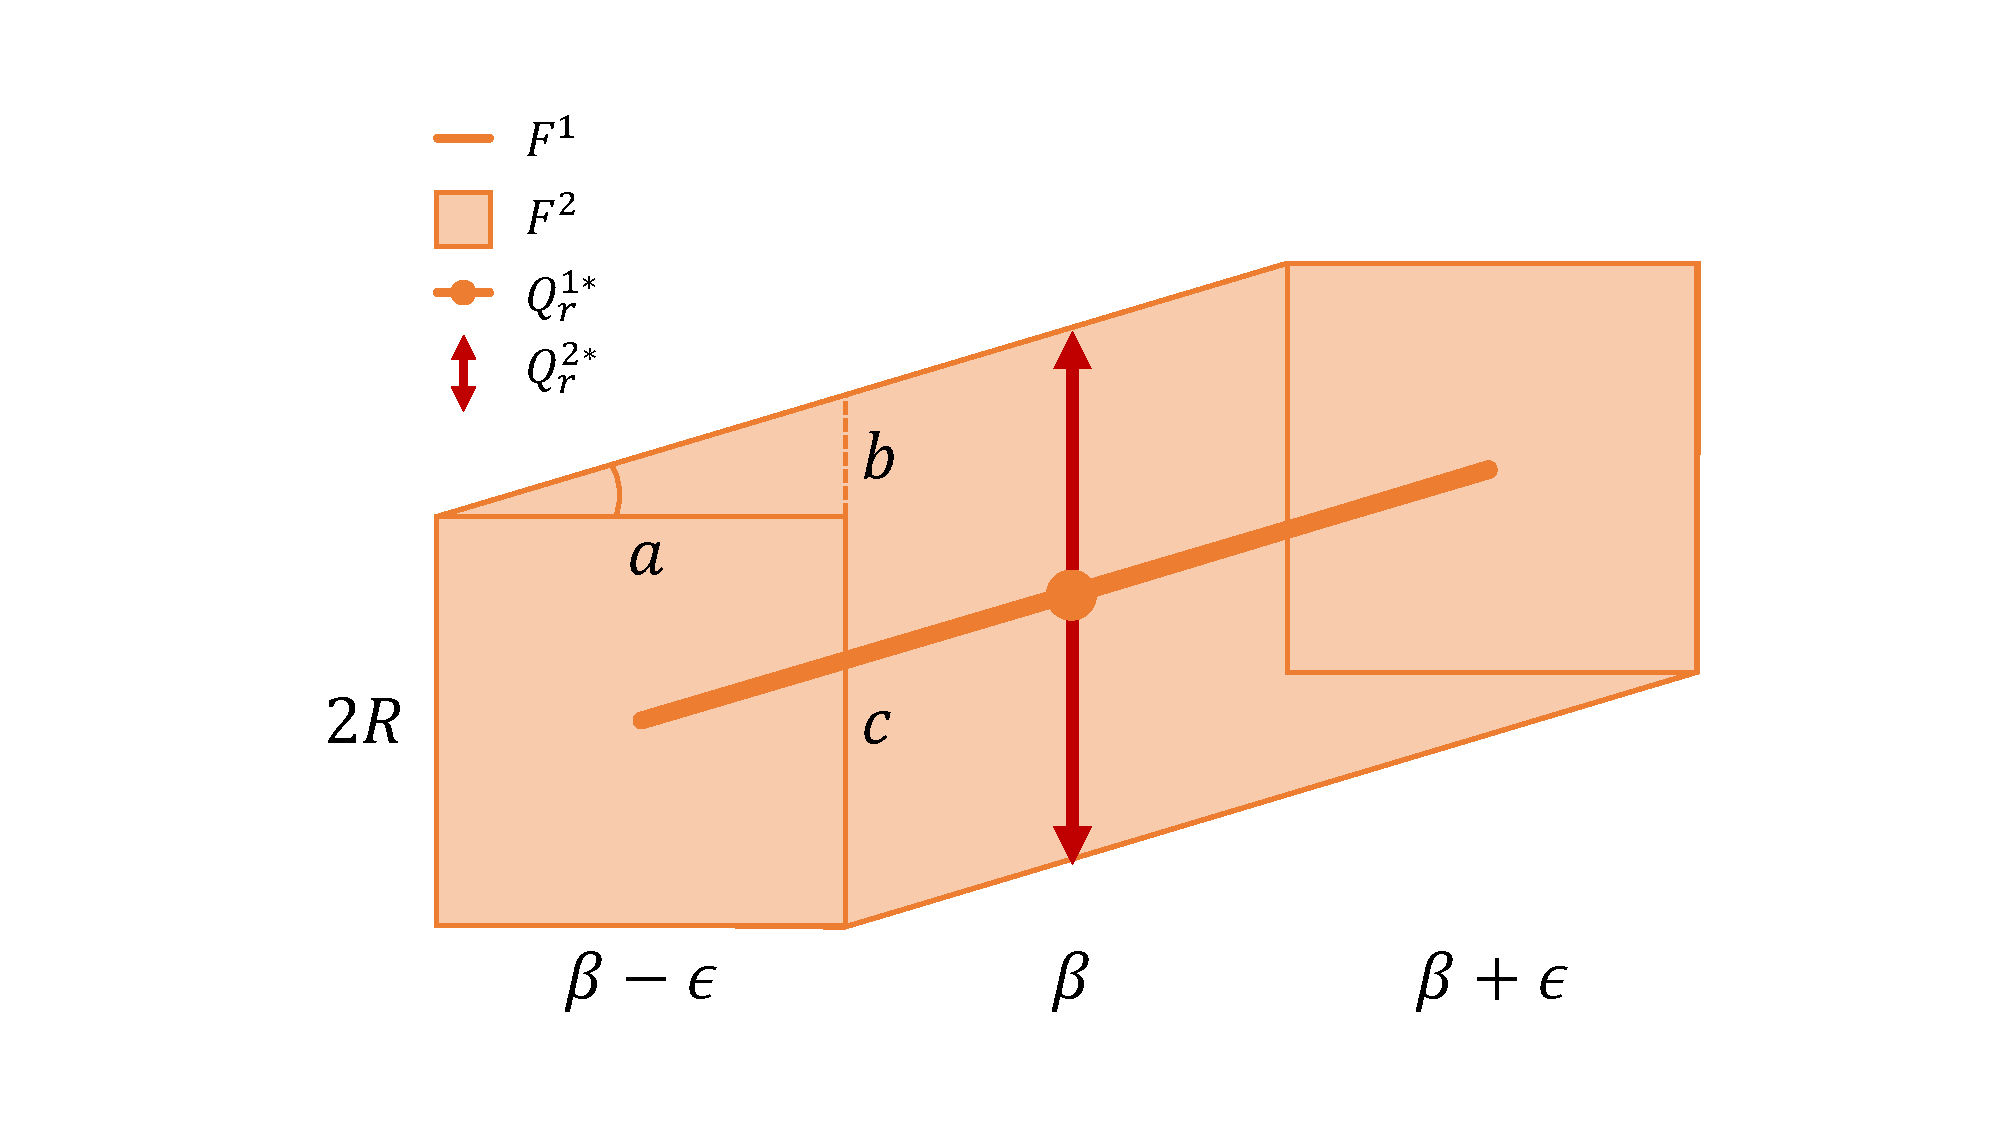
\includegraphics[trim=2cm 1cm 2cm 1cm, clip, width=0.7\textwidth]{source/img/contraction_lipschitz_slope.pdf}
    \caption{We represent a section $[\beta-\epsilon, \beta+\epsilon]$ of $\cF^1$ and $B(\cF^1, R)$. We want to bound the range of $Q_r^{2*}.$}
    \label{fig:contraction_lips_hull_slope}
\end{figure}

\begin{align*}
    \Delta Q_r^{2*} &= b + c &\\
    & \leq La + c & \text{($\cF^1$ $L$-Lipschitz)}\\
    &= 2LR+2R = 2R(L+1)
\end{align*}
Hence,
\begin{equation*}
    | Q_r^{2*} - Q_r^{1*}| \leq \frac{\Delta Q_r^{2*}}{2} = R(L+1)
\end{equation*}

and $Q_c^{1*} = Q_c^{2*} = \beta$.
Consequently, $ \|Q^{2*} - Q^{1*}\|_\infty \leq (L+1)R$

For completeness, the edge case in \Cref{sec:proof_pi_hull} should be considered as well.

\textbf{Wrapping it up:}

We've shown that for any $Q^1,Q^2\in\cL_\gamma$, and all $\os\in\ocS$, $\cF^2\in\cB(\cF^1,\|Q^2-Q^1\|_\infty)$ and $\cF^1$ is the graph of a $L$-Lipschitz function with $L<1/\gamma - 1$. Moreover, the solutions of $\pi_\text{greedy}(Q^1)$ and $\pi_\text{greedy}(Q^2)$ at $\os$ are such that $ \|Q^{2*} - Q^{1*}\|_\infty \leq (L+1)\|Q^2-Q^1\|_\infty$.

Hence, for all $\oa$,
\begin{align*}
    \|\cT Q^1(\os, \oa) - \cT Q^2(\os, \oa)\|_\infty &= \gamma\left\|\expectedvalueover{\os'\sim\ov{P}(\os'|\os,\oa)} \expectedvalueover{\oa'\sim\pi_\text{greedy}(Q^1)}Q^1(\os',\oa') - \expectedvalueover{\oa'\sim\pi_\text{greedy}(Q^2)}Q^2(\os',\oa')\right\|_\infty \\
    &= \gamma\left\|Q^{2*} - Q^{1*}\right\|_\infty \\
    &\leq \gamma(L+1)\|Q^2-Q^1\|_\infty
\end{align*}
Taking the sup on $\ocS\ocA$,

\begin{equation*}
    \|\cT Q^1 - \cT Q^2\|_\infty \leq \gamma(L+1)\|Q^1-Q^2\|_\infty
\end{equation*}
with $\gamma(L+1) < 1$.
As a conclusion, $\cT$ is a $\gamma(L+1)$-contraction on $\cL_\gamma$.
\end{proof}

%\subsection{Lemma \ref{lemma:concavity}}

%\begin{proof}. Let $s,s'\in\cS, a\in\cA$.
%We first prove those results for $V_r^*(s', \cdot)$

%\textbf{Non-decreasing}

%Consider $\beta_a^1 \leq \beta_a^2 \in \cB$.
%Any policy that satisfies the budget $\beta_a^1$ in $s'$ also satisfies $\beta_a^2$, so $\Pi_c(s', \beta_a^1) \subset \Pi_c(s', \beta_a^2)$. Hence, by taking the max over policies, $V_r^*(s', \beta_a^1) \leq V_r^*(s', \beta_a^2)$.
%Hence, $V_r^*(s', \cdot)$ is non-decreasing.

%\textbf{Concave}

%By contradiction: assume that $V_r^*(s', \cdot)$ is not concave, i.e. there exist $\beta^1 < \beta^2\in \cB$ and $p\in(0, 1)$ such that $\beta^3 = (1-p)\beta^1 + p\beta^2$ verifies: $V_r^*(s', \beta^3) < (1-p)V_r^*(s', \beta^1) + pV_r^*(s',\beta^2)$. By definition of $V^*$, there must be $\pi_1,\pi_2\in\Pi^*$ such that $V^*(s', \beta^1) = V^{\pi_1}(s', \beta^1)$ and $V^*(s', \beta^2) = V^{\pi_2}(s', \beta^2)$. 

%Define $\pi = (1-p)(\pi_1(\cdot, \beta^1), \pi_1) + p(\pi_2(\cdot, \beta^2), \pi_2)$. By linearity of $V^\pi$ with respect to $\pi$, we have that $V_c^\pi(s', \beta^3) = (1-p)V_c^{\pi_1}(s', \beta^1) + pV_c^{\pi_2}(s', \beta^2) \leq (1-p)\beta^1 + p\beta^2 = \beta^3$ since $\pi_1, \pi_2\in\Pi^*(s')\subset\Pi_a(s')$, so $\pi$ respects the budget $\beta^3$. Moreover, we also have $V_r^\pi(s', \beta^3) = (1-p)V_r^{\pi_1}(s', \beta^1) + pV_r^{\pi_2}(s', \beta^2) > V_r^*(s', \beta^3)$, which contradicts the definition of $V_r^*$.

%Consequently, $V_r^*(s', \cdot)$ is non-decreasing and concave. By \eqref{eq:bellman_expectation_Q} we see that $Q_r^*(s,a,\cdot) = R_r(s,a) + \gamma\expectedvalueover{s'}V_r^*(s', \cdot)$  is too.


%\end{proof}

%\subsection{Lemma \ref{lemma:tau_concavity}}


%\subsection{Lemma \ref{lemma:pi_hull}}

%\td

%\begin{proof}
%If the estimates $q^c_0, q^c_1$ are accurate, then by construction and linearity of the expectation, the returned mixture policy has an expected total cost of $\expectedvalueover{a, \beta_a \sim\pi_\text{greedy}}Q_c(s, a, \beta_a) = \beta$ as desired in \eqref{eq:pi_greedy_constraint}. Because the $Q_r(s,a,\cdot)$ is concave and under its tangents, this mixture must have the largest $Q_r$ possible as required in \eqref{eq:pi_greedy_reward}. The special case of a tie $q_r^0 = q_r^1$ is considered, where we do minimise $Q_c$ as required in \eqref{eq:pi_greedy_cost}.
%\end{proof}


\subsection{\Cref{prop:bftq_pi_hull}}
\label{sec:proof_pi_hull}
\begin{definition}
Let $A$ be a set, and $f$ a function defined on $A$. We define:

\begin{itemize}
    \item Convex hull of $A$: $\cC(A) = \{\sum_{i=1}^p \lambda_i a_i: a_i\in A, \lambda_i\in\Real^+, \sum_{i=1}^p \lambda_i = 1, p\in\Natural\}$
    \item Convex edges of $A$: $\cC^2(A) = \{\lambda a_1 + (1-\lambda)a_2: a_1, a_2\in A, \lambda\in[0, 1]\}$
    \item Dirac distributions of $A$: $\delta(A) = \{\delta(a-a_0): a_0\in A\}$ 
    \item Image of $A$ by $f$: $f(A) = \{f(a): a\in A\}$
\end{itemize}
\end{definition}

\begin{proof}
Let $\os=(s,\beta)\in\ocS$ and $Q\in(\Real^2)^{\ocS\ocA}$. We recall the definition of $\pi_\text{greedy}$:
\begin{subequations}
\begin{equation}
    \pi_\text{greedy}(\oa|\os; Q) \in \argmin_{\rho\in\Pi_r^Q} \expectedvalueover{\oa\sim\rho}Q_c(\os, \oa) \tag{\ref{eq:pi_greedy_cost}}
\end{equation}
\begin{align}
    \text{where }\quad\Pi_r^Q = &\argmax_{\rho\in\cM(\ocA)} \expectedvalueover{\oa\sim\rho} Q_r(\os, \oa) \tag{\ref{eq:pi_greedy_reward}}\\
    & \text{ s.t. }  \expectedvalueover{\oa\sim\rho} Q_c(\os, \oa) \leq \beta \tag{\ref{eq:pi_greedy_constraint}}
\end{align}
\end{subequations}

Note that any policy in the $\argmin$ in \eqref{eq:pi_greedy_cost} is suitable to compute $\cT$.
We first reduce the set of candidate optimal policies.
Consider the problem described in \eqref{eq:pi_greedy_reward},\eqref{eq:pi_greedy_constraint}: it can be seen as a single-step CMDP problem with reward $R_r=Q_r$ and cost $R_c=Q_c$. By \citep[Theorem 4.4][]{BEUTLER1985236}, we know that the solutions are mixtures of two deterministic policies. Hence, we can replace $\cM(\cA)$ by $\cC^2(\delta(\ocA))$ in \eqref{eq:pi_greedy_reward}.

Moreover, remark that:
\begin{align*}
    \{\expectedvalueover{\oa\sim\rho} Q(\os,\oa): \rho\in \cC^2(\delta(\ocA))\} &= \{\expectedvalueover{\oa\sim\rho} Q(\os,\oa): \rho=(1-\lambda)\delta(\oa-\oa_1)+\lambda\delta(\oa-\oa_2), \oa_1,\oa_2\in\ocA, \lambda\in[0,1]\} \\
    &= \{(1-\lambda)Q(\os, \oa_1)+\lambda Q(\os, \oa_2), \oa_1,\oa_2\in\ocA, \lambda\in[0,1]\} \\
    &= \cC^2(Q(\os,\ocA))\}
\end{align*}

Hence, the problem \eqref{eq:pi_greedy_reward}, \eqref{eq:pi_greedy_constraint} has become:
\begin{equation*}
    \tilde{\Pi}^Q_r = \argmax_{(q_r, q_c)\in\cC^2(Q(\os, \ocA))} q_r \quad\text{ s.t. }\quad q_c \leq \beta 
\end{equation*}
and the solution of $\pi_\text{greedy}$ is $q^*=\argmin_{q\in\tilde{\Pi}^Q_r} q_c$. 

The original problem in the space of actions $\ocA$ is now expressed in the space of values $Q(\os, \ocA)$ (which is why we use $=$ instead of $\in$ before $\argmin$ here).

We further restrict the search space of $q^*$ following two observations:
\begin{enumerate}
    \item $q^*$ belongs to the \emph{undominated} points $\cC^2(Q^-)$:
    \begin{align}
        \label{eq:q_minus_undominated}
        Q^+ &= \{(q_c, q_r): q_c > q_c^{\pm} = \min_{q^+} q_c^+\text{ s.t. }q^+\in\argmax_{q\in Q(\os,\ocA)} q_r\}\\
        Q^- &= Q(\os,\ocA) \setminus Q^+
    \end{align}
    Denote $q^*$ = $(1-\lambda) q^1 + \lambda q^2$, with $q^1, q^2\in Q(\os,\ocA)$. There are three possible cases:
    \begin{enumerate}
        \item $q^1, q^2 \not\in Q^-$. Then $q_c^* = (1-\lambda) q^1_c + \lambda q^2_c > q_c^{\pm}$. But then $q_c^{\pm} < q_c^* \leq \beta$ so $q^{\pm}\in\tilde{\Pi}^Q_r$ with a strictly lower $q_c$ than $q^*$, which contradicts the $\argmin$.
        \item $q^1\in Q^-, q^2 \not\in Q^-$. But then consider the mixture $q^\top = (1-\lambda) q^1 + \lambda q^\pm$. Since $q_r^{\pm} \geq q_r^{2}$ and $q_r^{\pm} < q_r^{2}$, we also have $q^\top_r \geq q_r^*$ and $q^\top_c < q_c^*$, which also contradicts the $\argmin$.
        \item $q^1,q^2\in Q^-$ is the only remaining possibility.
    \end{enumerate}
    \item $q^*$ belongs to the \emph{top frontier} $\cF$:
    \begin{equation*}
        \cF_Q = \{q\in \cC^2(Q^-): \not\exists q'\in \cC^2(Q^-): q_c=q_c'\text{ and }q_r<q_r'\}
    \end{equation*}
    Trivially, otherwise q' would be a better candidate than $q^*$.
\end{enumerate}


Let us characterise this frontier $\cF$. It is both:
\begin{enumerate}
    \item the \emph{graph of a non-decreasing function}: $\forall q^1, q^2\in\cF$ such that $q_c^1\leq q_c^2$ then $q_r^1\leq q_r^2$.\\
    By contradiction, if we had $q_r^1 > q_r^2$, we could define $q^\top = (1-\lambda)q^1 + \lambda q^\pm$ where $q^\pm$ is the dominant point as defined in \eqref{eq:q_minus_undominated}. By choosing $\lambda=(q^2_c-q^1_c)/(q^\pm_c-q^1_c)$ such that $q^\top_c = q_c^2$, then since $q_r^\pm \geq q_r^1 > q_r 2$ we also have $q^\top_r > q_r^2$ which contradicts $q^2\in\cF$.
    \item the \emph{graph of a concave function}: $\forall q^1, q^2, q^3\in\cF$ such that $q_c^1\leq q_c^2 \leq q_c^3$ with $\lambda$ such that $q^2_c = (1-\lambda)q^1_c + \lambda q^3_c$, then $q_r^2 \geq (1-\lambda)q_r^1 + \lambda q_r^3$.\\
    Trivially, otherwise the point $q^\top = (1-\lambda)q^1 + \lambda q^3$ would verify $q^\top_c=q^2_c$ and $q^\top_r > q^2_r$, which would contradict $q^2 \in\cF$.
\end{enumerate}

We denote $\cF_Q = \cF \cap Q$. Clearly, $q^*\in\cC^2(\cF_Q)$: let $q^1, q^2\in Q^-$ such that $q^* = (1-\lambda)q^1  + \lambda q^2$. First, $q^1, q^2\in Q^-\subset\cC^2(Q^-)$. Then, by contradiction, if there existed $q^{1'}$ or $q^{2'}$ with equal $q_c$ and strictly higher $q_r$, again we could build an admissible mixture $q^{\top}=(1-\lambda)q^{1'}  + \lambda q^{2'}$ strictly better than $q^*$.

$q^*$ can be written as $q^* = (1-\lambda)q^1  + \lambda q^2$ with $q^1, q^2\in\cF_Q$ and, without loss of generality, $q^1_c \leq q^2_c$.

\textbf{Regular case:} there exists $q^0\in\cF_Q$ such that $q^0_c \geq \beta$.

Then $q^1$ and $q^2$ must flank the budget: $q_c^1 \leq \beta \leq q_c^2$. Indeed, by contradiction, if $q_c^2 \geq q_c^1 > \beta$ then $q_c^* > \beta$ which contradicts $\Pi_r^Q$. Conversely, if $q_c^1 \leq q_c^2 < \beta$ then $q^* < \beta \leq q^0_c$, which would make $q^*$ a worse candidate than $q^\top=(1-\lambda)q^* + \lambda q^0$ when $\lambda$ is chosen such that $q_c^\top=\beta$, and contradict $\Pi_r^Q$ again.

Because $\cF$ is the graph of a non-decreasing function, $\lambda$ should be as high as possible, as long as the budget $q^*\leq\beta$ is respected. We reach the highest $q_r^*$ when $q^*_c=\beta$, that is: $\lambda=(\beta-q_c^1)/(q_c^2-q_c^1)$.

It remains to show that $q^1$ and $q^2$ are two successive points in $\cF_Q$: $\not\exists q\in\cF_Q\setminus\{q^1, q^2\}: q^1_c \leq q_c \leq q^2_c$. Otherwise, as $\cF$ is the graph of a concave function, we would have $q_r \geq (1-\mu)q_r^1 + \mu q_r^2$. $q_r$ cannot be strictly greater than $(1-\mu)q_r^1 + \mu q_r^2$ which would contradict $q^*$, but it can still be equal, which means the tree points $q, q^1, q^2$ are aligned. In fact, every points aligned with $q^1$ and $q^2$ can also be used to construct mixtures resulting in $q^*$, but among these solutions we can still choose $q^1$ and $q^2$ as the two points in $\cF_Q$ closest to $q^*$.

\textbf{Edge case:} $\forall q\in\cF_Q, q_c < \beta$. Then  $q^* =  \argmax_{q\in\cF} q_r = q^\pm =  \argmax_{q\in Q^-} q_r$

\end{proof}


%\begin{proof}
%First, a straightforward proof by induction shows that for all $k\in\Natural$, $Q_k$ computed at iteration $k$ of either Algorithm \ref{algo:bvi} or Algorithm \ref{algo:bftq} is concave non-decreasing with respect to $\beta_a$: the initialisation is trivial from $Q_0 = 0$, and the heredity stems from Lemma \ref{lemma:tau_concavity}.
%\end{proof}


% \subsection{Decomposition Lemma}

% \begin{lemma}
%     For any sequence real valued functions $f_1,\ldots,f_n$ and any real number $c$, we have:
%     \[
%         \begin{array}{lcl}
%             \underbrace{\max\limits_{\sum_i x_i \leq c}\sum_j f_j(x_j)}_{(a)} & \quad{}=\quad{} & \underbrace{\max\limits_{\sum_i c_i \leq c}\left(\sum_j\max\limits_{x\leq c_j} f_j(x)\right)}_{(b)}\\
%         \end{array}
%     \]
% \end{lemma}

% \begin{proof}
%     Let us first show that $(a)\leq(b)$.
%     By definition of the maximum on a set, for any $f_j$ and any $c_j$ we have:
%     $\max\limits_{x\leq c_j} f_j(x) \geq f_j(c_j)$.
%     Hence, by replacing these terms in $(b)$ we get:
%       \[
%     \begin{array}{lcl}
%         \max\limits_{\sum_i c_i \leq c} \sum_j f_j(c_j) & \quad{}\leq\quad{} & \max\limits_{\sum_i c_i\leq c}\left(\sum_j \max\limits_{x_j\leq c_j} f_j(x_j)\right)\\
%     \end{array}
%     \]
%     The left hand side of this inequality is just a rewriting of $(a)$ with different dummy variables names.

%     Let us show now that $(a) \geq (b)$.
%     Let $\hat{x}_1,\ldots,\hat{x}_n, \hat{c}_1, \ldots \hat{c}_n$ be a realisation (argmax) of $(b)$.
%     By definition of $(b)$'s feasible set, we have $\sum_i\hat{c}_i \leq c$ and for any $i$: $\hat{x}_i\leq \hat{c}_i$.
%     Because $\sum_i\hat{x}_i\leq \sum_i\hat{c}_i \leq c$, the tuple $(\hat{x}_1, \ldots \hat{x}_n)$ is also a feasible value for $(a)$. And, by definition of the maximum on a set: $(a) = \max\limits_{\sum_i x_i \leq c} \sum_j f_j(x_j) \geq \sum_j f_j(\hat{x}_j) = (b)$.
% \end{proof}

\section{Risk-Sensitive Exploration}
\label{sec:risk-sensitive-supp}
We recall the Risk-Sensitive Exploration algorithm in \Cref{algo:risk-sensitive-exploration}


\begin{algorithm}[H]
\DontPrintSemicolon
\KwData{An environment, a BFTQ solver, $W$ CPU workers}
\KwResult{A batch of transitions $\cD$}
$\cD\leftarrow\{\}$\;
\For{each intermediate batch} {
split episodes between $W$ workers\;
\For(\tcp*[f]{run this loop on each worker in parallel}){each episode in batch}{
sample initial budget $\beta\sim\mathcal{U}(\mathcal{B})$.\;
\While{episode not done}{
update $\epsilon$ from schedule.\;
sample $z\sim\mathcal{U}([0, 1])$.\;
\lIf{$z < \epsilon$}{sample $(a, \beta_a)\sim\mathcal{U}(\Delta_{\cA\cB})$.\tcp*[f]{Explore}}
\lElse{sample $(a, \beta_a)\sim\pi_\text{greedy}(a, \beta_a|s, \beta; Q^*)$.\tcp*[f]{Exploit}}
append transition $(s, \beta, a, \beta_a, R, C, s')$ to batch $\mathcal{D}$.\;
step episode budget $\beta \leftarrow \beta_a$
}
}
$\pi_\text{greedy}(\cdot\sim; ~Q^*) \leftarrow\texttt{BFTQ}(\cD)$.
}
\Return{the batch of transitions $\cD$}
%     \STATE 
%     \WHILE{episode not done}
%     \STATE Update $\epsilon$ from schedule.
%     \STATE Sample $z\sim\mathcal{U}([0, 1])$.
%     \IF {$z > \epsilon$}
%     \STATE Sample $(a, \beta')$ from $(\pi_\mathcal{A}, \pi_\mathcal{B})$. \COMMENT{Exploit}
%     \ELSE
%     \STATE Sample ($a$, $\beta'$) from $\mathcal{U}(\Delta_{\mathcal{A}\mathcal{B}})$. \COMMENT{Explore}
%     \ENDIF
%     \STATE Append transition $(s, \beta, a, r', c', s')$ to batch $\mathcal{D}$.
%     \STATE Update episode budget $\beta \leftarrow \beta'$.
%     \ENDWHILE
%     \ENDFOR
%     \STATE $(\pi_\mathcal{A}, \pi_\mathcal{B}) \leftarrow\texttt{BFTQ}(\mathcal{D})$.
%     \ENDFOR
%     \STATE \textbf{return} the batch of transitions $\mathcal{D}$
\caption{Risk-sensitive exploration}
\label{algo:risk-sensitive-exploration}
\end{algorithm}

\section{Scalable Implementation of BFTQ}
\label{sec:bftq-full}

We recall the scalable version of BFTQ in \Cref{algo:bftq_full} and the architecture of the neural network \Cref{fig:architecture}.

%\begin{minipage}[t]{0.5\textwidth}
\begin{figure}[tp]
    \centering
    
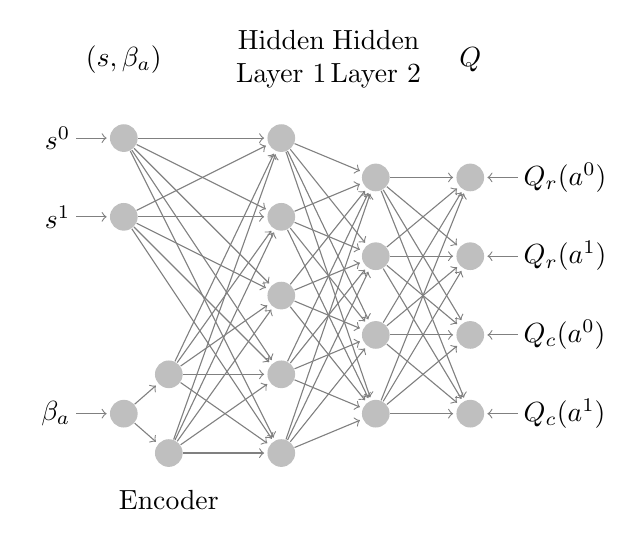
\begin{tikzpicture}[shorten >=1pt,->,draw=black!50, inner sep=1pt, node distance=\layersep]
        \tikzstyle{every pin edge}=[<-,shorten <=1pt]
        \tikzstyle{neuron}=[circle,fill=black!25,minimum size=10pt,inner sep=0pt]
        \tikzstyle{input neuron}=[neuron];
        \tikzstyle{input beta}=[neuron];
        \tikzstyle{qc}=[neuron];
        \tikzstyle{qr}=[neuron];
        \tikzstyle{hidden neuron}=[neuron];
        \tikzstyle{autoencoder neuron}=[neuron];
        \tikzstyle{annot} = [text width=4em, text centered]
        \tikzstyle{annot2} = [text width=10em, text centered]
        \def\layersep{2cm}
        % Draw the input layer nodes
        \foreach \name / \y in {0,...,1}
            \pgfmathtruncatemacro{\y}{0 + \y}
            \node[input neuron, pin=left:$s^\y$] (I-\name) at (0,-\y) {};

         % first layer
        \foreach \name / \y in {0,...,4}
        \pgfmathtruncatemacro{\y}{0 + \y}
            \path node[hidden neuron] (H1-\name) at (1*\layersep,-\y cm) {};

        \foreach \source in {0,...,1}
            \foreach \dest in {0,...,4}
                \path (I-\source) edge (H1-\dest);

        % BETA
        \node[input beta, pin=left:$\beta_a$] (BETA) at (0,-3.5) {};

        % beta auto encoder
        \foreach \name / \y in {0,...,1}
            \pgfmathtruncatemacro{\ybis}{3+ \y}
            \path node[autoencoder neuron] (AE-\name) at (\layersep/3.5,-\ybis cm) {};



        \foreach \name / \y in {0,...,3}
        \pgfmathtruncatemacro{\y}{0 + \y}
            \path[yshift=-0.5cm]
            node[hidden neuron] (H2-\name) at (1.6*\layersep,-\y cm) {};


        % actions
        \foreach \name / \y in {0,...,1}
        \pgfmathtruncatemacro{\y}{0 + \y}
            \path[yshift=-0.5cm] node[qr,pin=right:$Q_r(a^\y)$] (Qr-\name) at (2.2*\layersep,-\y cm) {};

        \foreach \name / \y in {0,...,1}
        \pgfmathtruncatemacro{\yy}{2 + \y}
            \path[yshift=-0.5cm] node[qc,pin=right:$Q_c(a^\y)$] (Qc-\name) at (2.2*\layersep,-\yy cm) {};

        \foreach \source in {0,...,1}
            \foreach \dest in {0,...,4}
                \path (AE-\source) edge (H1-\dest);



        \foreach \dest in {0,...,1}
            \path (BETA) edge (AE-\dest);

         \foreach \source in {0,...,4}
            \foreach \dest in {0,...,3}
                \path (H1-\source) edge (H2-\dest);

        \foreach \source in {0,...,3}
            \foreach \dest in {0,...,1}
                \path (H2-\source) edge (Qr-\dest);

         \foreach \source in {0,...,3}
            \foreach \dest in {0,...,1}
                \path (H2-\source) edge (Qc-\dest);
        % Annotate the layers
       \node[annot] (input) at (0,1) {$(s,\beta_a)$};
       \node[annot2] (input) at (\layersep/3.5,-4.6) {Encoder};
       \node[annot](h1) at (\layersep,1) {Hidden Layer 1};
       \node[annot](h2) at(1.6* \layersep,1) {Hidden Layer 2};
       \node[annot](output) at(2.2* \layersep,1) {$Q$};
        %\node[annot,right of=hl] {Output layer};
    \end{tikzpicture}

    \caption{Neural Network for $Q$-functions approximation when $\cS=\Real^2$ and $|\cA| = 2$.}
    \label{fig:architecture}
\end{figure}
%\end{minipage}

\begin{algorithm}[tp]
\DontPrintSemicolon
\KwData{$\mathcal{D}$, $\tilde{\mathcal{B}}$ a finite subset of $\mathcal{B}$, $\gamma$, a model $Q\in (\Real^2)^{S \ocA}$, a regression algorithm \texttt{fit}, a set of CPU workers $W$}
\KwResult{$Q^*$}
$Q \leftarrow 0$\;
$X \leftarrow \{s_i,a_i,\beta_{a_i}\}_{i\in[0, |\cD|]}$\;
$S' \leftarrow \{s_i'\}_{i\in[0, |\cD|]}$\;
\Repeat{convergence}{
   Evaluate $Q(S', \cA, \tilde{\cB})$ in a single forward pass\;
   Split $\mathcal{D}$ among workers: $\mathcal{D} = \cup_{w\in W} \mathcal{D}_w$\;
   \For(\tcp*[f]{Run in parallel}){$w\in W$}{
       \For{$(\boldsymbol{\cdot},\boldsymbol{\cdot},\beta_{a_i},{R_r}_i,{R_c}_i,s'_i) \in \mathcal{D}$} {
           $\cP \leftarrow \{(Q_c(s_i',\cA,\tilde{\cB}), Q_r(s_i',\cA,\tilde{\cB}))\}$\;
           $\cH \leftarrow \texttt{convex\_hull}(\cP).\text{vertices}()$\tcp*[f]{in cw order}\;
           $\cH.\texttt{prune}()$ \tcp*[f]{Remove all dominated points}\;
           $k \leftarrow \min\{k: \beta_i \geq q_c$ with $\left(q_c,q_r\right) = \cH[k]\}$\;
           $q_c^2,q_r^2,q_c^1,q_r^1 \leftarrow \cH[k],\cH[k-1]$\;
           $p \leftarrow (\beta_{a_i} - q_a^1) / (q_c^2 - q_c^1)$\;
           $Y_c^{w,i} \leftarrow {R_c}_i + \gamma ((1-p) q_c^1+ p q_c^2)$\;
           $Y_r^{w,i} \leftarrow {R_r}_i + \gamma ((1-p) q_r^1+ p q_r^2)$\;
       }
   }
   Join the results: $Y \leftarrow \cup_{w\in W} (Y_c^w, Y_r^w)$\;
   $Q \leftarrow \texttt{fit}(X, Y)$\;
}
\caption{Scalable BFTQ}
\label{algo:bftq_full}
\end{algorithm}

\section{The Lagrangian Relaxation Baseline}
\label{sec:lagragian}
As explained on \Cref{fig:Lagrangian}, the optimal deterministic policy can be obtained by a line-search on the Lagrange multiplier values $\lambda$.

Then, according to \citet[Theorem 4.4]{BEUTLER1985236}, the optimal policy is a randomised mixture of two deterministic policies: the safest deterministic policy that violates the constraint $\pi_{\lambda-}$ and the riskier of the feasible ones $\pi_{\lambda+}$.

Fitted-Q (FTQ)~\citep{Ernst2005,Riedmiller2005} can be easily adapted for continuous states CMDP and BMDP through this methodology, but given the high variance it requires a lot of simulations to get a proper estimate of the calibration curve. Our purpose is to avoid this calibration phase.

\begin{figure}[tp]
    \centering
    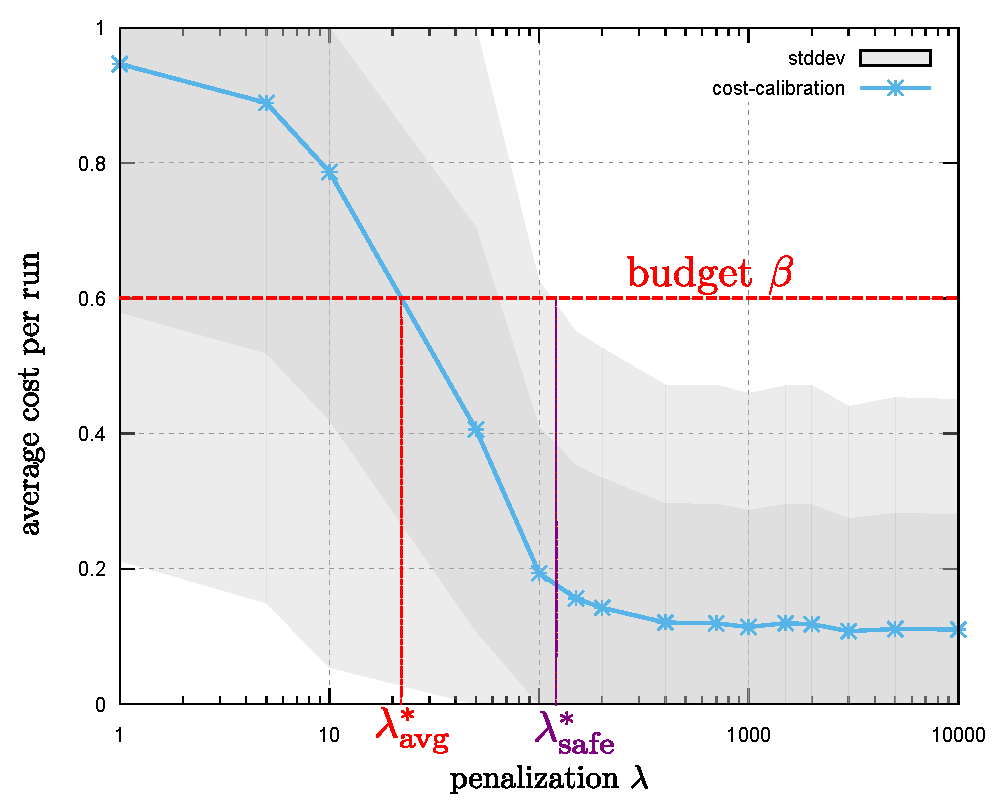
\includegraphics[width=0.5\textwidth]{source/img/CalibrationExample}
    \caption{Calibration of a penalty multiplier according to the budget $\beta$. The optimal multiplier $\lambda^*_{\text{avg}}$ is the smallest one to satisfy the budget constraint on average. Safer policies can also be selected according to the largest deviation from this mean cost.}
    \label{fig:Lagrangian}
\end{figure}


\section{Experiments}
\label{sec:exp-supp}


\subsection{Examples of different exploration strategies}
\label{subsec:exploration-examples}
We compare two approaches for constructing a batch of samples. The animations from the html page \url{exploration.html} display the trajectories collected in each intermediate sub-batch. The first row corresponds to a classical  risk neutral epsilon-greedy exploration policy while the second row showcases a risk-sensitive exploration strategy introduced in the paper. Each animation corresponds to a different seed.

\subsection{Examples of BFTQ policies executions}
\label{sec:bftq-executions}

We display the evolution in the budgeted policy behaviour with respect to the budget on different environments. The policies have been learnt with a risk-sensitive exploration.

\paragraph{Highway-Env}

On the \texttt{highway-env} , the budgeted agents display a wide variety of behaviours. Animations are displayed on the html page \url{highway-env.html}. When $\beta = 1$, the ego-vehicle drives in a very aggressive style: it immediately switches to the opposite lane and drives as fast as possible to pass slower vehicles, swiftly changing lanes to avoid incoming traffic. On the contrary when $\beta = 0$, the ego-vehicle is conservative: it stays on its lane and drives at a low velocity. With intermediate budgets such as $\beta = 0.2$, the agent sometimes decides to overtake its front vehicle but promptly steers back to its original lane afterwards.

\paragraph{Slot-filling}

\paragraph{Remark on the \texttt{slot-filling} environment} When receiving an utterance, the system can either understand it $(\mu=\mu_u)$ or misunderstand it $(\mu=\mu_m)$ with a fixed probability called the sentence error rate $ser$. Then, the speech recognition score is simulated \citep{Khouzaimi2015}: $srs = (1+\exp(-x))^{-1}$ with $x\sim N(\mu, \sigma)$. It's the confidence score of the natural language understanding module about the last utterance. Note that here are no recognition errors ($ser=0$ and $srs=1$) when the user provides information using the numeric pad.

In \Cref{table:dialogues}, we display two dialogues done with the same BFTQ policy on \texttt{slot-filling}. The policy is given two budgets to respect in expectation, $\beta=0$ and $\beta=0.5$. For $\beta=0$, one can see that the system never uses the \texttt{ask\_num\_pad} action. Instead, it uses \texttt{ask\_oral} , an action subject to recognition errors. The system keeps asking for the same slot 2, because it has the lowest speech recognition score. It eventually summarises the form to the user, but then reaches the maximum dialogue length and thus faces a dialogue failure. For $\beta=0.5$, the system first asks in a safe way, with \texttt{ask\_oral}. It may want to \texttt{ask\_num\_pad} if one of the speech recognition score is low. Then, the system proceeds to a confirmation of the slot values. If it is incorrect, the system continues the dialogue using unsafe the \texttt{ask\_num\_pad} action to be certain of the slot values.

\begin{table}[H]
\centering
\resizebox{\textwidth}{!}{
\begin{tabular}[]{lll}
\toprule

turn&$\beta=0$&$\beta=0.5$\tabularnewline
\midrule
turn 0& \makecell[l]{valid slots : [0, 0, 0]\\ srs : [ None None None ]\\ system says ASK\_ORAL(1) \\ user says INFORM} &\makecell[l]{ valid slots : [0, 0, 0]\\ srs : [ None None None ]\\ system says ASK\_ORAL(2)\\ user says INFORM}\tabularnewline\midrule
turn 1&\makecell[l]{valid slots : [0, 0, 0]\\ srs : [ None 0.48 None ]\\ system says ASK\_ORAL(2) \\ user says INFORM} & \makecell[l]{valid slots : [0, 0, 1]\\ srs : [ None None 0.56 ]\\ system says ASK\_ORAL(0)\\ user says INFORM}\tabularnewline\midrule
turn 2&\makecell[l]{valid slots : [0, 0, 0]\\ srs : [ None 0.48 0.22 ]\\ system says ASK\_ORAL(0) \\ user says INFORM} & \makecell[l]{valid slots : [0, 0, 1] \\ srs : [ 0.30 None 0.56 ]\\ system says ASK\_ORAL(1)\\ user says INFORM}\tabularnewline\midrule
turn 3&\makecell[l]{valid slots : [0, 0, 0]\\ srs : [ 0.62 0.48 0.22 ]\\ system says ASK\_ORAL(2) \\ user says INFORM} & \makecell[l]{valid slots : [0, 0, 1]\\ srs : [ 0.30 0.54 0.56 ]\\ system says ASK\_ORAL(0)\\ user says INFORM}\tabularnewline\midrule
turn 4&\makecell[l]{valid slots : [0, 0, 0] \\ srs : [ 0.62 0.48 0.66 ]\\ system says ASK\_ORAL(1) \\ user says INFORM} & \makecell[l]{valid slots : [0, 0, 1]\\ srs : [ 0.68 0.54 0.56 ]\\ system says ASK\_NUM\_PAD(1)\\ user says INFORM}\tabularnewline\midrule
turn 5&\makecell[l]{valid slots : [0, 1, 0]\\ srs : [ 0.62 0.56 0.66 ]\\ system says ASK\_ORAL(2) \\ user says INFORM} & \makecell[l]{valid slots : [0, 1, 1]\\ srs : [ 0.68 1.00 0.56 ]\\ system says SUMMARIZE\_AND\_INFORM\\ user says DENY\_SUMMARIZE}\tabularnewline\midrule
turn 6&\makecell[l]{valid slots : [0, 1, 0]\\ srs : [ 0.62 0.56 0.14 ]\\ system says ASK\_ORAL(2) \\ user says INFORM} & \makecell[l]{valid slots : [0, 1, 1]\\ srs : [ 0.68 1.00 0.56 ]\\ system says ASK\_NUM\_PAD(2)\\ user says INFORM}\tabularnewline\midrule
turn 7&\makecell[l]{valid slots : [0, 1, 1]\\ srs : [ 0.62 0.56 0.30 ]\\ system says ASK\_ORAL(2) \\ user says INFORM }& \makecell[l]{valid slots : [0, 1, 1]\\ srs : [ 0.68 1.00 1.00 ]\\ system says SUMMARIZE\_AND\_INFORM\\ user says DENY\_SUMMARIZE}\tabularnewline\midrule
turn 8&\makecell[l]{valid slots : [0, 1, 1]\\ srs : [ 0.62 0.56 0.49 ]\\ system says ASK\_ORAL(2) \\ user says INFORM} & \makecell[l]{valid slots : [0, 1, 1]\\ srs : [ 0.68 1.00 1.00 ]\\ system says ASK\_NUM\_PAD(0)\\ user hangs up !}\tabularnewline\midrule
turn 9&\makecell[l]{valid slots : [0, 1, 1]\\ srs : [ 0.62 0.56 0.65 ]\\ system says SUMMARIZE\_AND\_INFORM \\ max size reached !}& \makecell[l]{ }\tabularnewline\bottomrule
\end{tabular}
}
    \caption{Two dialogues generated by a safe policy ($\beta=0$) on the left and a risky one ($\beta=0.5$) on the right.}
    \label{table:dialogues}
\end{table}

\paragraph{Corridors}

Animations are displayed on the html page \url{corridors.html} for the \texttt{corridors} environment. When the budget is low, the agent takes the safest path on the left. When the budget increases, it gradually switches to the other lane, earning higher rewards but also costs. This gradual process could not be achieved with a deterministic policy as it would chose either one path or the other. Each animation corresponds to a different seed.

\subsection{Reproducibility}
\label{subsec:reproducibility-supp}

The following section displays environments and algorithms parameters and instructions to reproduce the exact same results displayed in \Cref{sec:experiements}.

\subsubsection{Environments Parameters}
\label{sec:env-parameters}

All environments parameters are displayed in \Cref{tab:param-corridors}, \Cref{tab:param-slot-filling} and \Cref{tab:param-highway-env}.


\paragraph{State-Space}

The states $s$ (from $\os=(s,\beta)$) of the agent are described in the following:

\begin{itemize}
    \item \texttt{Corridors}: $s = (x,y)$ where $x$ and $y$ are the 2D coordinates of the agent.
    \item \texttt{Slot-Filling}: $s = (\text{srs},\text{min},a_u,a_s,t)$ where $\text{srs}$ is a vector of the speech recognition score for each slot, $\text{min}$ is a one hot vector describing the minimum of the $\text{srs}$ vector, $a_u$ is a one hot vector of the last user dialogue act and $a_s$ is the one hot vector of the last system dialogue act. Finally $t\in[0,1]$ is the fraction of the current turn with the maximum number of turns authorised.
    \item \texttt{Highway-Env}: the positions $(x, y)$ and velocities $(\dot{x}, \dot{y})$ of every vehicle on the road.
\end{itemize}


\begin{table}[ht!]
    \centering
    \begin{tabularx}{1.0\textwidth}{lll}
        \toprule
        Parameter & Description & Value\tabularnewline
        \midrule
        - & Size of the environment & 7 x 6\tabularnewline
        - & \makecell[l]{Standard deviation of the Gaussian \\noise applied to actions} & (0.25,0.25)\tabularnewline
        H & Episode duration & 9\tabularnewline
        \bottomrule
    \end{tabularx}
    \caption{Parameters of \texttt{Corridors}}
    \label{tab:param-corridors}
\end{table}

\begin{table}[ht!]
    \centering
    \begin{tabularx}{1.0\textwidth}{lll}
        \toprule
        Parameter & Description & Value\tabularnewline
        \midrule
        ser & Sentence Error Rate & 0.6\tabularnewline
        $\mu_m$& Gaussian mean for misunderstanding & -0.25\tabularnewline
        $\mu_u$& Gaussian mean for understanding & 0.25\tabularnewline
        $\sigma$& Gaussian standard deviation & 0.6\tabularnewline
        $p$& Probability of hang-up & 0.25\tabularnewline
        H & Episode duration & 10\tabularnewline
        - & Number of slots & 3\tabularnewline
        \bottomrule
    \end{tabularx}
    \caption{Parameters of \texttt{Slot-Filling}}
    \label{tab:param-slot-filling}
\end{table}


\begin{table}[ht!]
    \centering
    \begin{tabularx}{1.0\textwidth}{lll}
        \toprule
        Parameter & Description & Value\tabularnewline
        \midrule
        $N_v$& Number of vehicles & 2 - 6\tabularnewline
        $\sigma_p$& Standard deviation of vehicles initial positions & 100 m\tabularnewline
        $\sigma_v$& Standard deviation of vehicles initial velocities & 3 m/s\tabularnewline
        H & Episode duration & 15 s\tabularnewline
        \bottomrule
    \end{tabularx}

    \caption{Parameters of \texttt{highway-env}}
    \label{tab:param-highway-env}
\end{table}

\subsubsection{Algorithm parameters}
\label{sec:algorithms-parameters}

All algorithm parameters are displayed in \Cref{tab:param-algo-corridors},\Cref{tab:param-algo-slot-filling} and \Cref{tab:param-algo-highway-env}.

\paragraph{A note on the parameters search}

We performed a shallow grid-search for the classic Neural-Network parameters. Most of the parameters don't have a strong influence on the results, however in the \texttt{slot-filling} environment, the choice of the regulation weight is decisive.

\begin{table}[tp]
    \centering
    \begin{tabularx}{1.0\textwidth}{lll}
        \toprule
        Parameters & BFTQ(risk-sensitive) & BFTQ(risk-neutral)\tabularnewline
        \midrule
        architecture & 256x128x64 & 256x128x64\tabularnewline
        regularisation & 0.001 & 0.001\tabularnewline
        activation & relu & relu\tabularnewline
        size beta encoder & 3 & 3\tabularnewline
        initialisation & xavier & xavier\tabularnewline
        loss function & L2 & L2\tabularnewline
        optimizer & adam & adam\tabularnewline
        learning rate & 0.001 & 0.001\tabularnewline
        epoch (NN) & 1000 & 5000\tabularnewline
        normalize reward & true & true\tabularnewline
        epoch (FTQ) & 12 & 12\tabularnewline
        $\tilde{\cB}$ & 0:0.01:1 & -\tabularnewline
        $\gamma$ & 1 & 1\tabularnewline
        $N=|\cD|$ & 5000 & 5000\tabularnewline
        $N_\text{minibatch}$ & 10 & 10\tabularnewline
        $N_\text{seeds}$ & 4 & 4\tabularnewline
        $N_\text{test}$ & 1000 & 1000\tabularnewline
        decay epsilon scheduling & 0.001 & 0.001\tabularnewline
        \bottomrule

    \end{tabularx}
    \caption{Algorithms parameters for \texttt{Corridors}}
    \label{tab:param-algo-corridors}
\end{table}

\begin{table}[tp]
    \centering
    \begin{tabularx}{1.0\textwidth}{lll}
        \toprule
        Parameters & BFTQ & FTQ\tabularnewline
        \midrule
        architecture & 256x128x64 & 128x64x32\tabularnewline
        regularisation & 0.0005 & 0.0005\tabularnewline
        activation & relu & relu\tabularnewline
        size beta encoder & 50 & -\tabularnewline
        initialisation & xavier & xavier\tabularnewline
        loss function & L2 & L2\tabularnewline
        optimizer & adam & adam\tabularnewline
        learning rate & 0.001 & 0.001\tabularnewline
        epoch (NN) & 5000 & 5000\tabularnewline
        normalize reward & true & true\tabularnewline
        epoch (FTQ) & 11 & 11\tabularnewline
        $\tilde{\cB}$ & 0:0.01:1 & -\tabularnewline
        $\gamma$ & 1 & 1\tabularnewline
        $N=|\cD|$ & 5000 & 5000\tabularnewline
        $N_\text{minibatch}$ & 10 & 10\tabularnewline
        $N_\text{seeds}$ & 6 & 6\tabularnewline
        $N_\text{test}$ & 1000 & 1000\tabularnewline
        decay epsilon scheduling & 0.001 & 0.001\tabularnewline
        \bottomrule
    \end{tabularx}
    \caption{Algorithms parameters for \texttt{Slot-Filling}}
    \label{tab:param-algo-slot-filling}
\end{table}
\begin{table}[tp]
    \centering
    \begin{tabularx}{1.0\textwidth}{lll}
        \toprule
        Parameters & BFTQ & FTQ\tabularnewline
        \midrule
        architecture & 256x128x64 & 128x64x32\tabularnewline
        regularisation & 0.0005 & 0\tabularnewline
        activation & relu & relu\tabularnewline
        size beta encoder & 50 & -\tabularnewline
        initialisation & xavier & xavier\tabularnewline
        loss function & L2 & L2\tabularnewline
        optimizer & adam & adam\tabularnewline
        learning rate & 0.001 & 0.01\tabularnewline
        epoch (NN) & 5000 & 400\tabularnewline
        normalize reward & true & true\tabularnewline
        epoch (FTQ) & 15 & 15\tabularnewline
        $\tilde{\cB}$ & 0:0.01:1 & -\tabularnewline
        $\gamma$ & 0.9 & 0.9\tabularnewline
        $N=|\cD|$ & 10000 & 10000\tabularnewline
        $N_\text{minibatch}$ & 10 & 10\tabularnewline
        $N_\text{seeds}$ & 10 & 10\tabularnewline
        $N_\text{test}$ & 150 & 150\tabularnewline
        decay epsilon scheduling & 0.0003 & 0.0003\tabularnewline
        \bottomrule
    \end{tabularx}
    \caption{Algorithms parameters for \texttt{Highway-Env}}
    \label{tab:param-algo-highway-env}
\end{table}

\subsubsection{Instructions for reproducibility}
\label{subsubsec:instruction-reproducibility}
To reproduce the result displayed in \Cref{sec:experiements}, first install the following conventional libraries for python3: pycairo, numpy, scipy and pytorch. Then, execute the commands in \Cref{fig:instructions} on a Linux Operating System. The Graphic Processing Unit used for experiments is an NVIDIA \texttt{GeForce GTX 1080 Ti} and the Computational Processing Unit is an Intel \texttt{Xeon E7}.

\begin{figure}
    \centering
    

\begin{minted}{sh}
# Install highway-env
pip3 install --user git+https://github.com/eleurent/rl-agents
# Change python path to the path of this repository
export PYTHONPATH="code/scaling-up-brl"
# Navigate to budgeted-rl folder
cd code/scaling-up-brl/budgeted-rl/
# Run main script using any config file
# Choose the range of seeds you want to test on
python3 main/egreedy/main-egreedy.py config/slot-filling.json 0 6
python3 main/egreedy/main-egreedy.py config/corridors.json 0 4
python3 main/egreedy/main-egreedy.py config/highway-easy.json 0 10
\end{minted}
\caption{Instructions to reproduce experiments}
    \label{fig:instructions}
\end{figure}


\section{The machine learning reproducibility checklist}
\label{sec:ml-checklist}
For all models and algorithms presented, indicate if you include: 

\begin{itemize}
    \item  A clear description of the mathematical setting, algorithm, and/or model:
    
    \begin{itemize}\item \textbf{yes}, see \Cref{sec:intro}, \Cref{sec:bdp}, \Cref{sec:brl},
    \Cref{sec:risk-sensitive-supp} and \Cref{sec:bftq-full}.
    \end{itemize}
    \item An analysis of the complexity (time, space, sample size) of any algorithm:
    \begin{itemize}\item \textbf{yes}, see \Cref{subsec:parallel-computing}.
    \end{itemize}
    \item A link to a downloadable source code, with specification of all dependencies, including external libraries:
    \begin{itemize}\item \textbf{yes}, see \Cref{subsubsec:instruction-reproducibility} and the folder \texttt{code} in the supplementary material zip file.
    \end{itemize}
\end{itemize}

For any theoretical claim, indicate if you include:

\begin{itemize}
    \item  A statement of the result:
     \begin{itemize}
        \item  \textbf{yes}, see \Cref{sec:bdp} and \Cref{sec:brl}.\end{itemize}
    \item A clear explanation of any assumptions:
    \begin{itemize}
        \item  we make one assumption in \Cref{sec:bdp}. We assume the program is feasible for any state. If not, no algorithm would be able to solve it anyway.\end{itemize}
    \item A complete proof of the claim:
    \begin{itemize}
        \item  \textbf{yes}, see \Cref{sec:proofs}. We formulate a conjecture in \Cref{rmk:contractivity-smooth} but we provide a sketch of the proof in \Cref{proof:contraction-with-smooth}.\end{itemize}
\end{itemize}

For all figures and tables that present empirical results, indicate if you include:

\begin{itemize}
    \item A complete description of the data collection process, including sample size: 
    
        \begin{itemize}
            \item\textbf{yes}, see \Cref{sec:experiements} and \Cref{sec:algorithms-parameters}.
        \end{itemize}
    \item A link to a downloadable version of the dataset or simulation environment:
    
        \begin{itemize}
            \item  \textbf{yes}, two environments   are shipped with the supplementary material (in the \texttt{code} folder) and the third one is fetch from a public repository, see \Cref{subsubsec:instruction-reproducibility} for details.
        \end{itemize}
    \item An explanation of any data that were excluded, description of any pre-processing step: 
        \begin{itemize}
            \item it's \textbf{not applicable} as data comes from simulated environments, so pre-processing steps are not needed.
        \end{itemize}

    \item An explanation of how samples were allocated for training / validation / testing: 
        \begin{itemize}
            \item it's \textbf{not applicable}. The complete dataset is used for training. There is no need for validation set. Testing is performed in the true environment as in classical online learning approaches.
        \end{itemize}

    \item The range of hyper-parameters considered, method to select the best hyper-parameter configuration, and specification of all hyper-parameters used to generate results: 
    
        \begin{itemize}
            \item \textbf{yes}, see \Cref{sec:algorithms-parameters}.
        \end{itemize}

    \item The exact number of evaluation runs: 
    
        \begin{itemize}
            \item \textbf{yes}, see $N_{seeds}$ in the tables from \Cref{sec:algorithms-parameters}.
        \end{itemize}

    \item A description of how experiments were run:              \begin{itemize}
            \item \textbf{yes}, see the two first paragraphs of \Cref{par:ex-explo}.
        \end{itemize}

    \item A clear definition of the specific measure or statistics used to report results:
        \begin{itemize}
            \item  \textbf{yes}, see \Cref{subsec:results}.
        \end{itemize}

    \item Clearly defined error bars:
    
        \begin{itemize}
            \item  \textbf{yes}, we plot 95\% confidence intervals in all figures, see \Cref{subsec:results}.
        \end{itemize}

    \item A description of results with central tendency (e.g. mean)  variation (e.g. stddev):
    
        \begin{itemize}
            \item  \textbf{yes}, we even observe less variability with our novel approach, see \Cref{subsec:results}.
        \end{itemize}
    \item A description of the computing infrastructure used:     \begin{itemize}
            \item The Graphic Processing Unit used for experiments is an NVIDIA \texttt{GeForce GTX 1080 Ti} and the Computational Processing Unit is an Intel \texttt{Xeon E7}.
        \end{itemize}
\end{itemize}